\Section{Signal Modifier Parameter Inference with cINNs}

In this chapter, the performance of the network will be characterized in detail. Two network setups will be considered: one without and one with a summary network reducing the representation of the conditions. These networks will be referred to cINN and SN-cINN (for summary network-extended cINN). It will be shown that the setup without a summary network results in superior performance for which an explanation will be given. 

\Subsection{Training Performance}

The evolution of the loss functions are shown in fig. \ref{fig:losses}. The location of the models with the lowest validation loss is shown with the red dashed line; the corresponding loss values are $-5.16$ for the cINN and $-4.96$ for the SN-cINN. It becomes clear at first glance the SN-cINN models suffer from overtraining -- no network from the three independent runs with different initializations have converged during training. This effect has also been observed in \cite{Ksoll_2020}. The structure of the summary network has been chosen in a way that this network had the lowest validation loss; models with a deeper summary network or less output nodes tend to produce worse results with a higher loss. Fortunately, the predictions are of the same quality if the summary network architecture is suitably chosen.

\begin{figure}[h!]
	\begin{minipage}{.5\textwidth}
		\centering
		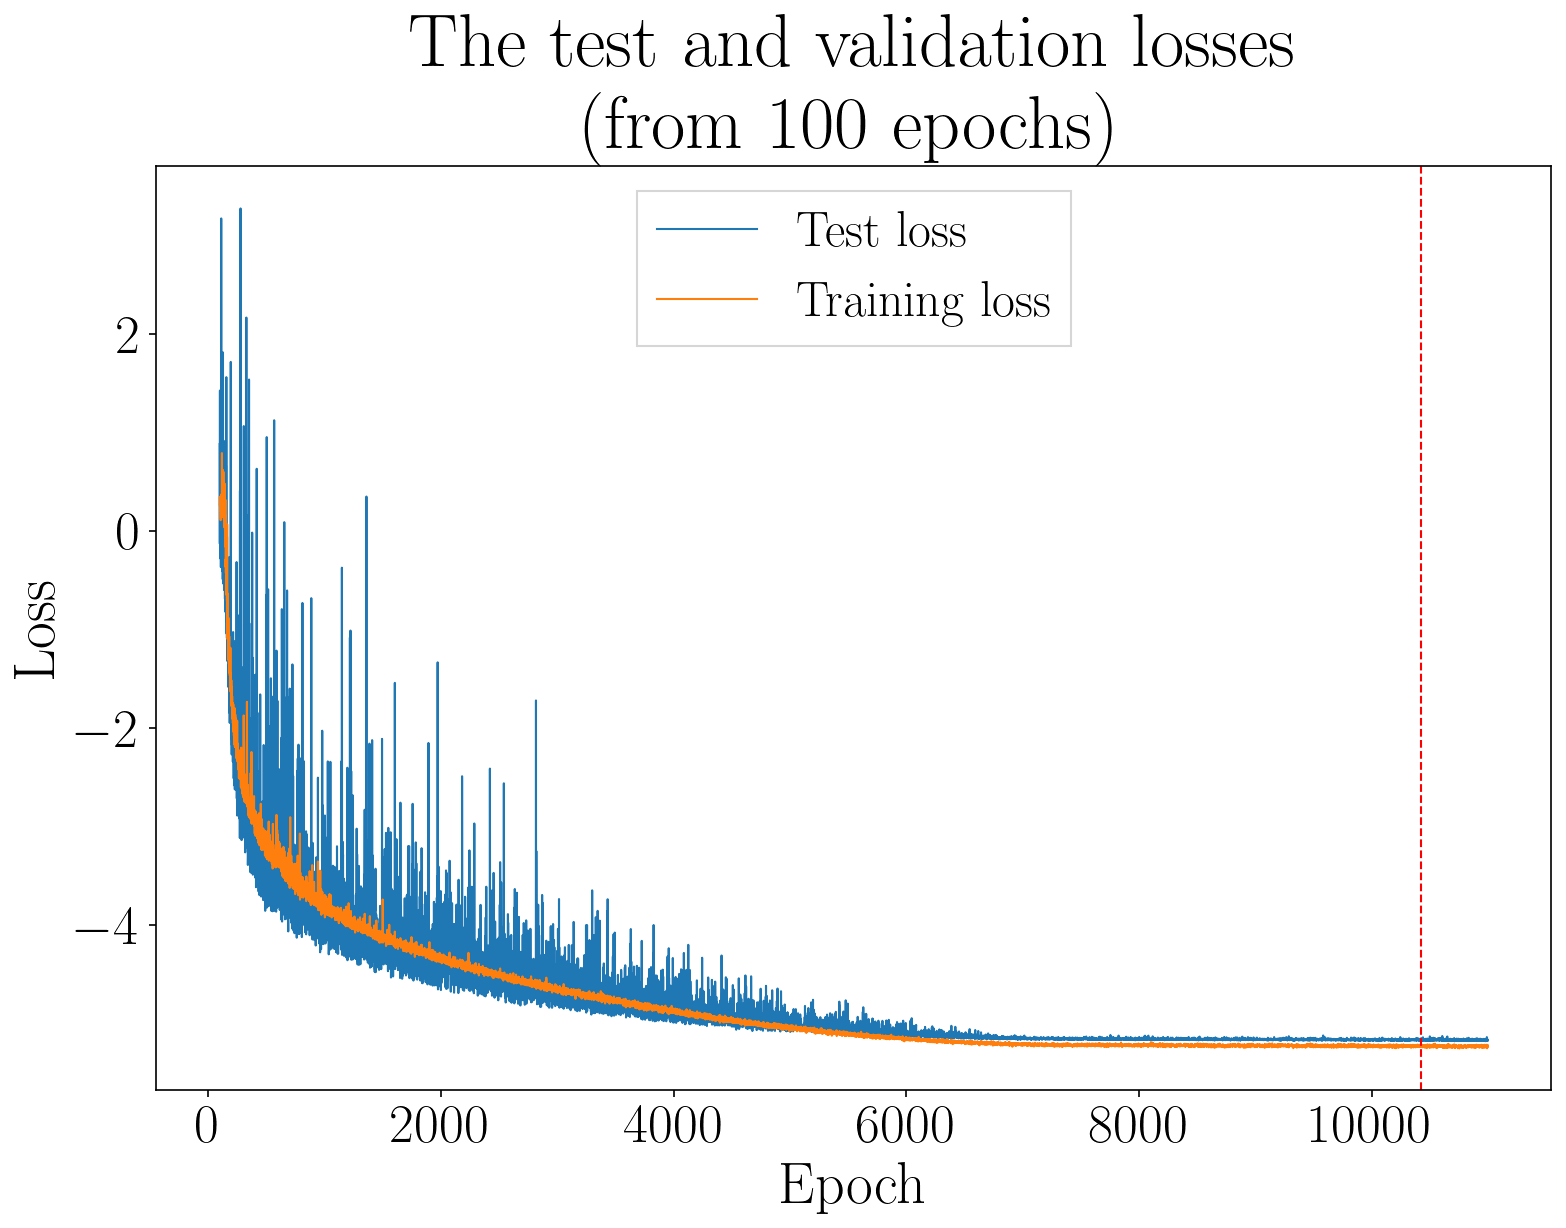
\includegraphics[width=\linewidth]{figures/inference/losses}
	\end{minipage}%
	\begin{minipage}{.5\textwidth}
		\centering
		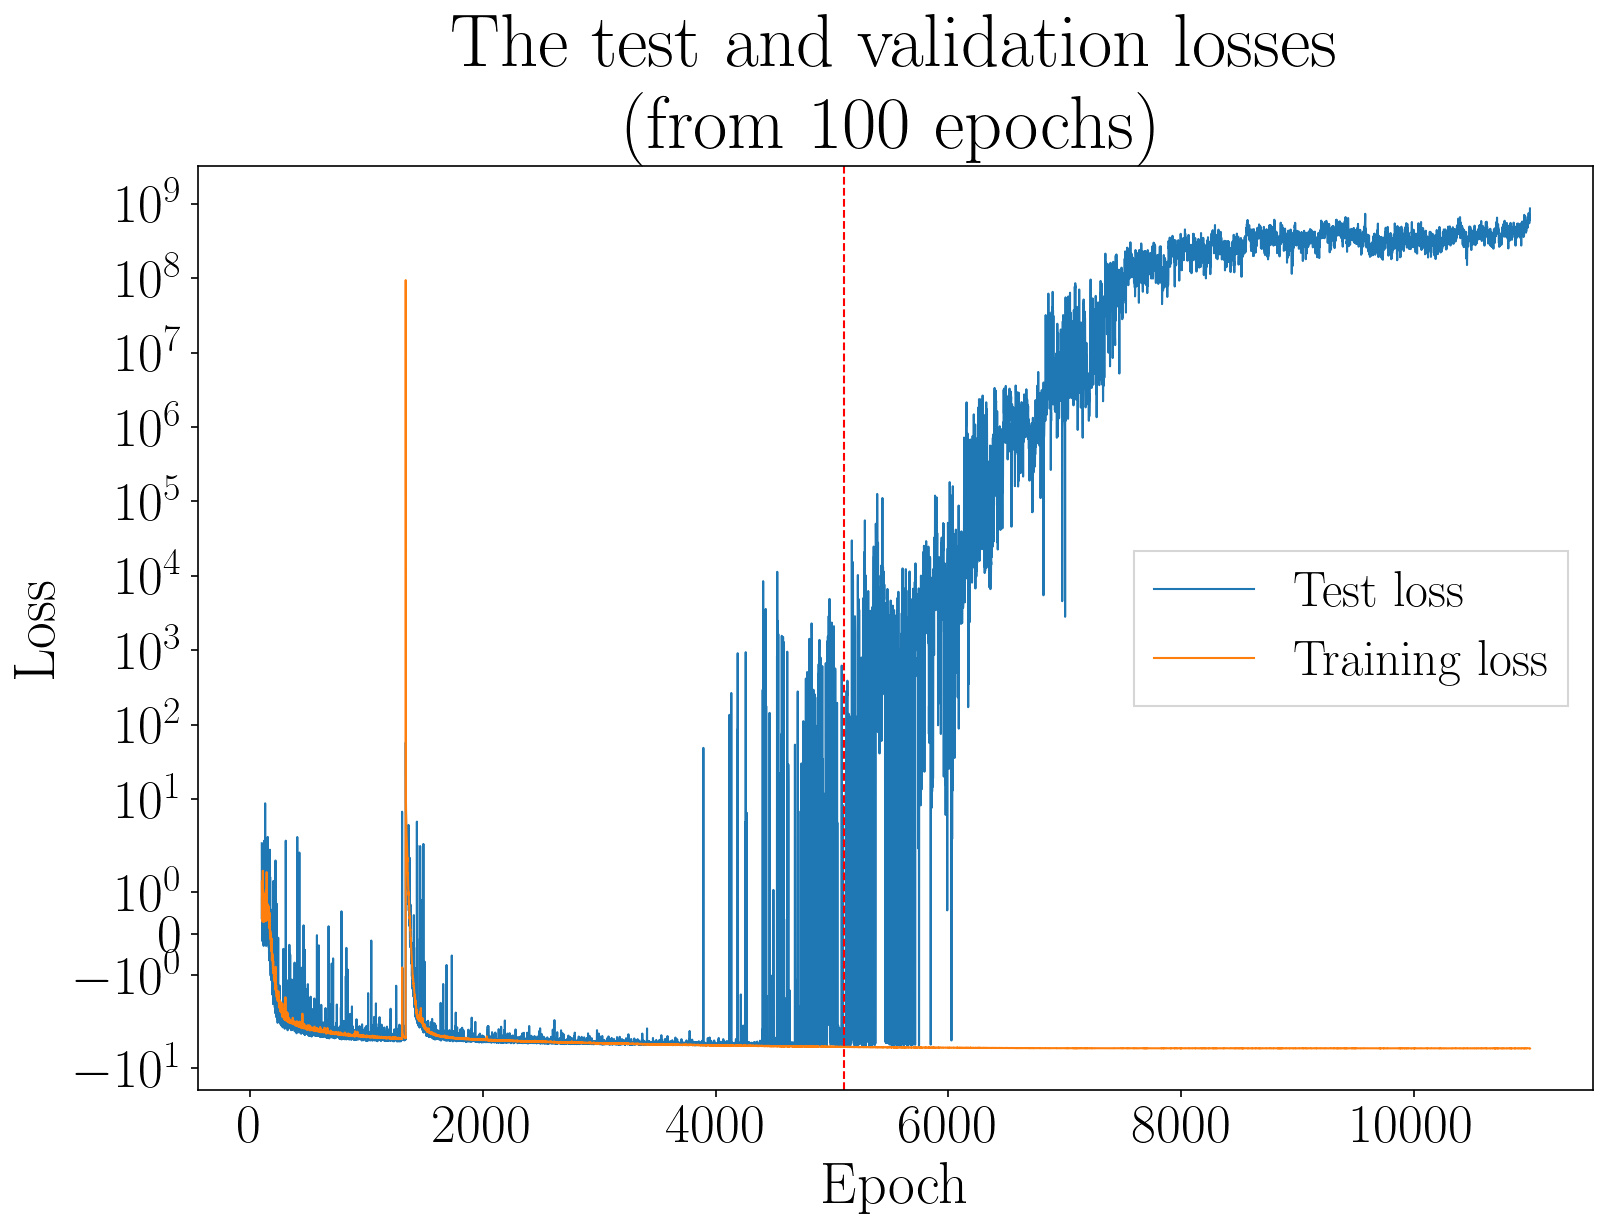
\includegraphics[width=\linewidth]{figures/inference/losses_SN}
	\end{minipage}
	\centering
	\caption{The loss values for each network from the 100th epoch (initial losses cut off as they disturb the graph) for the cINN and for the SN-cINN. Models with the lowest validation loss are shown with the red dashed line. Note the overtraining for the summary network (right)}
	\label{fig:losses}
\end{figure}

From the losses it becomes clear that the condition dimensionality cannot be significantly reduced as each input bin carries the same value of information as these are uncorrelated among themselves. For this reason, the reduction of the conditions necessarily result in performances of lower quality.

\Subsection{\textcolor{red}{Latent Space Distribution}}

At the end of chapter \ref{ch:deeplearning}, the loss function has been constructed in a way that the input variables should be mapped to a multivariate normal distribution with $\mu = 0$ and $\Sigma=1$. Note that thanks to the Universal Approximation Theorem, the diffeomorphic mappings in the normalizing flow represented by the GLOW coupling blocks can be approximated arbitrary well for a well-constructed network architecture and well-chosen optimization procedure. Since loss functions per se do not carry any information about the quality of the resulting mapping, the shape of the network output -- the latent space distribution -- serves as a suitable candidate to check whether there are any issues with the setup.

The latent space distribution for both networks are shown if fig. \ref{fig:latents} for the models with the lowest test loss. The distribution of the datapoints are shown in the blue histograms while a normal function with mean 0 and standard deviaiton 1 is shown in orange.

\begin{figure}[h!]
	\centering
	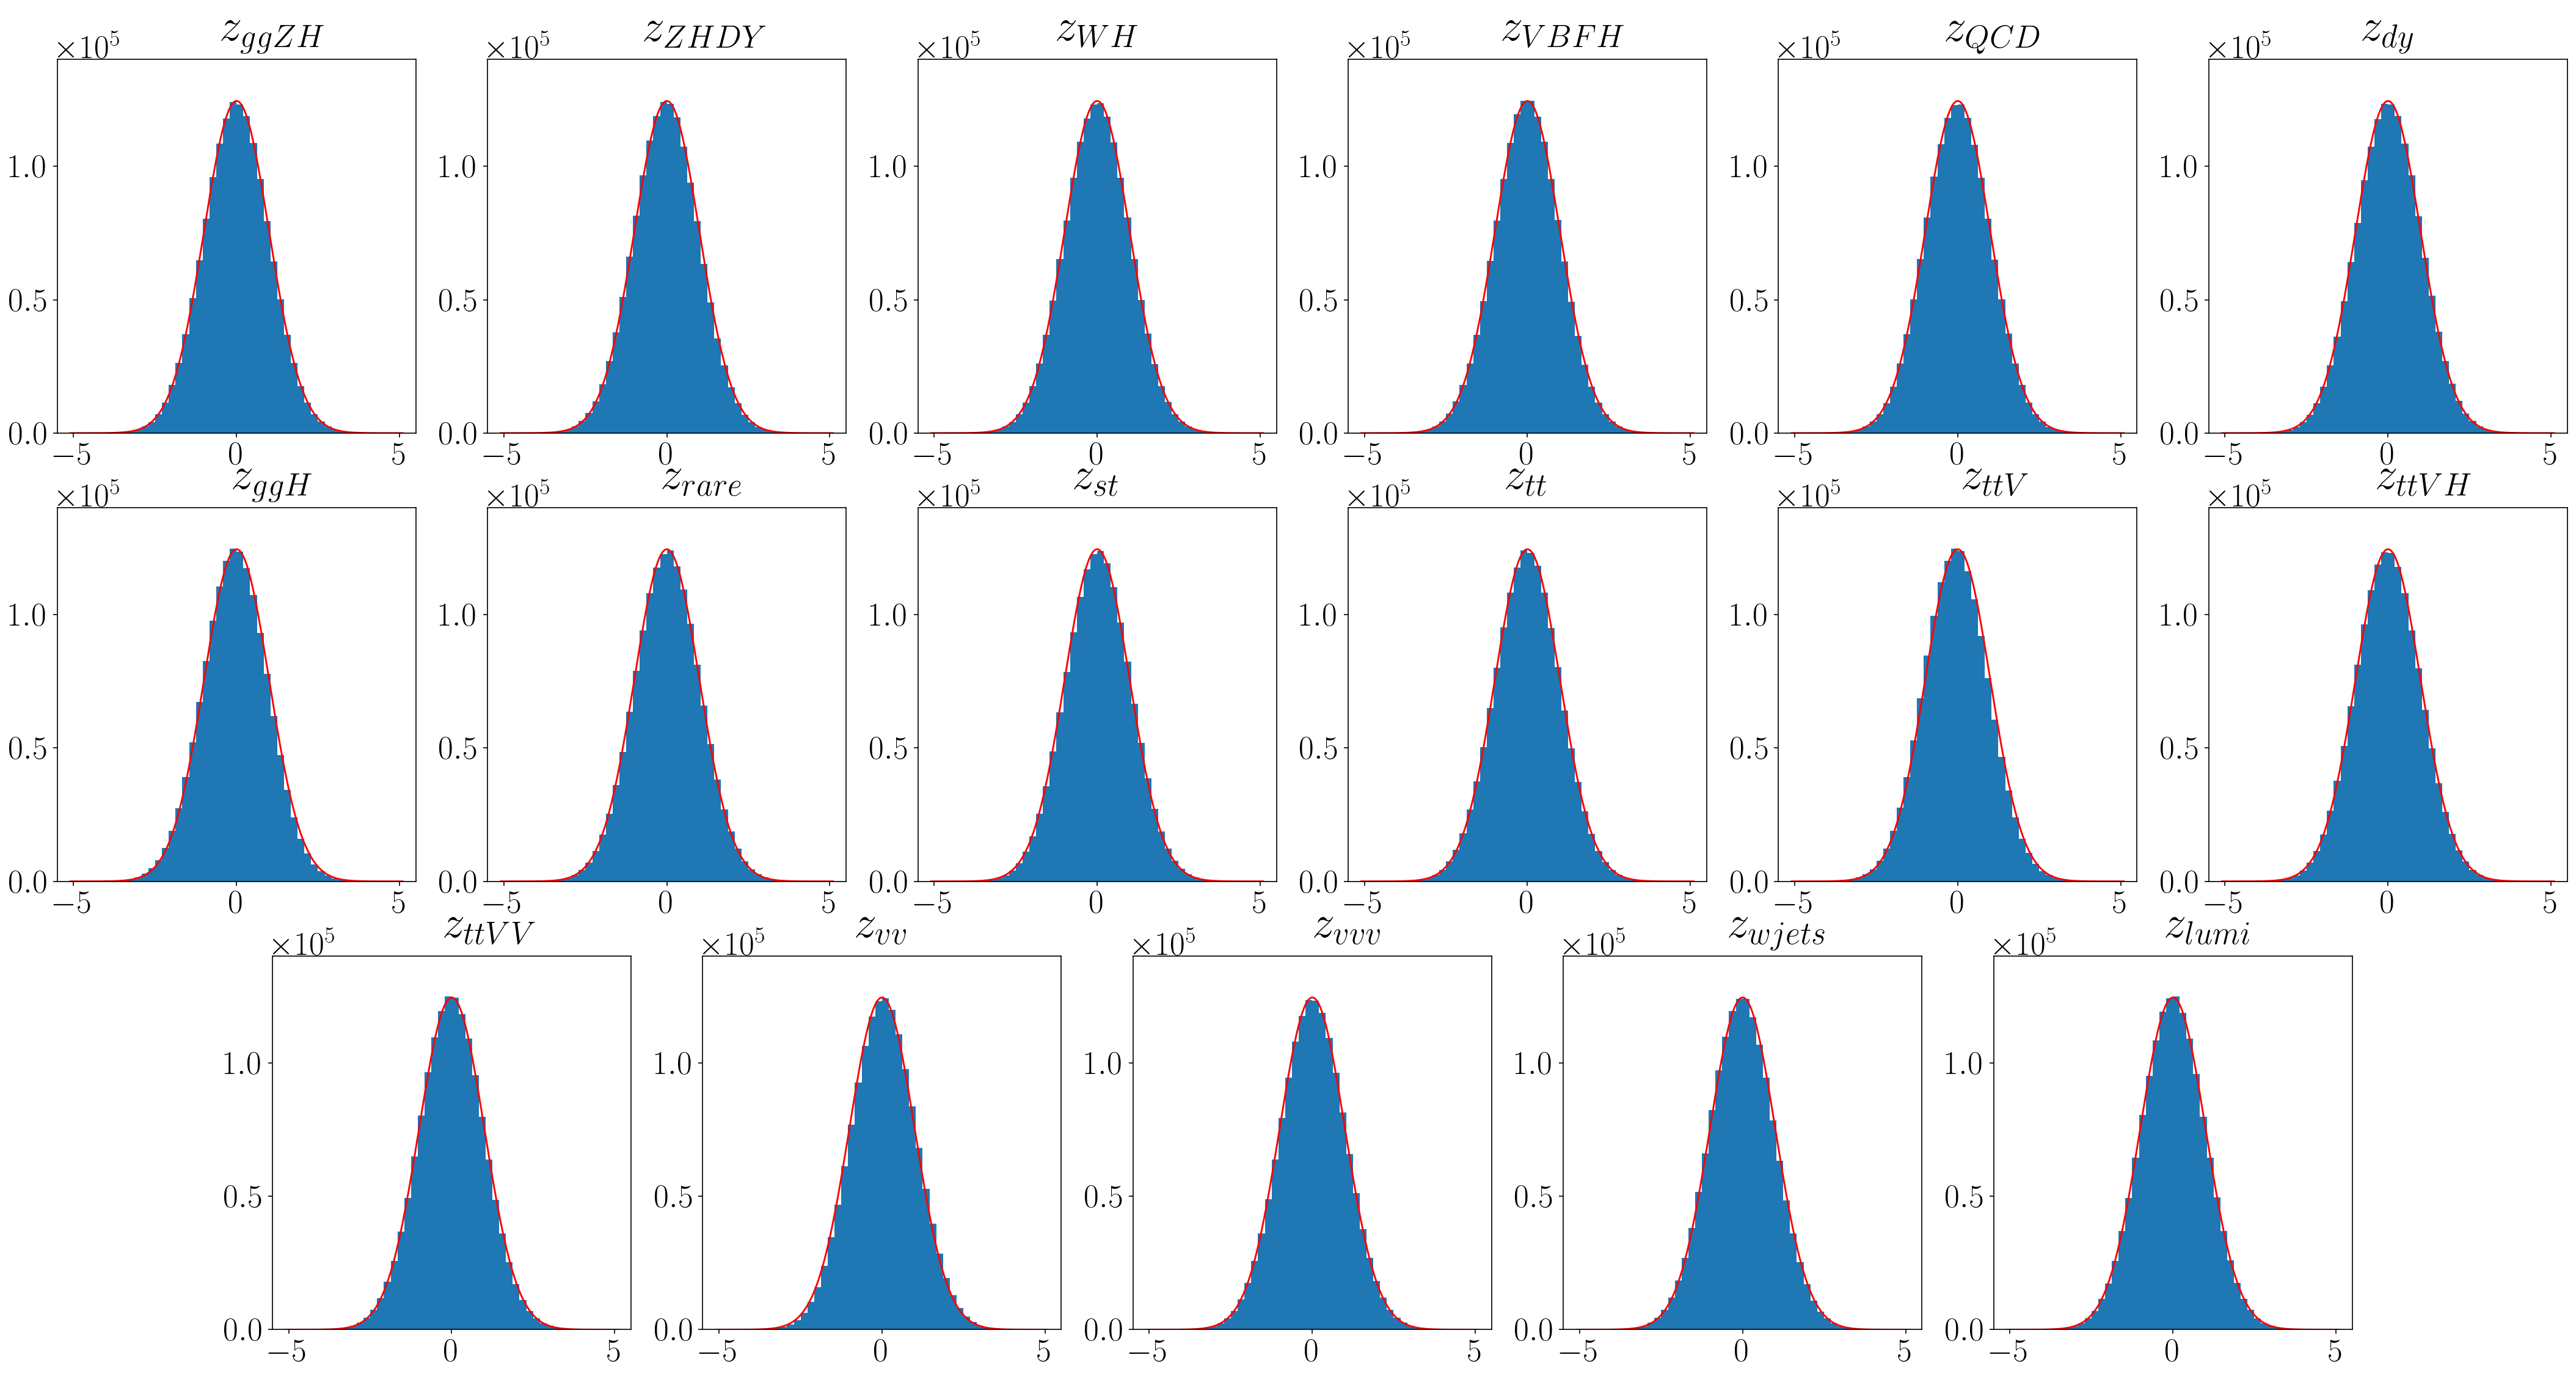
\includegraphics[width=\textwidth]{figures/inference/ls.png}
	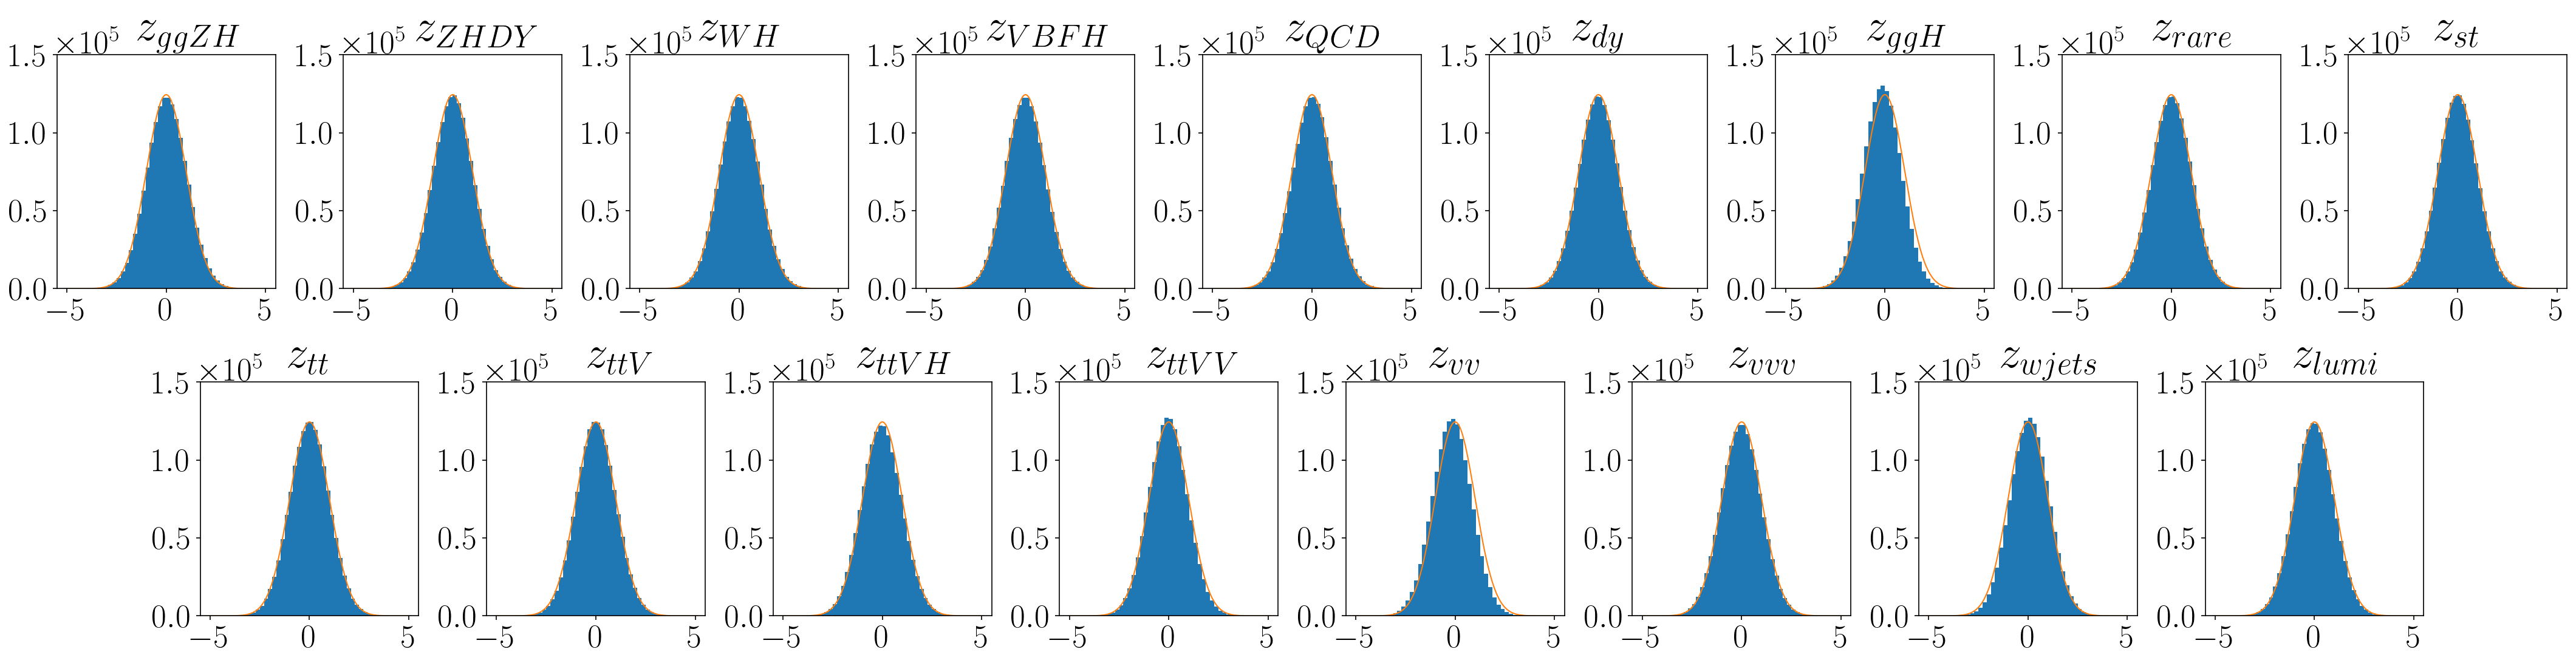
\includegraphics[width=\textwidth]{figures/inference/ls_SN.png}
	\caption{Latent space distribution for the cINN without (top) and with (bottom) a summary network.\textcolor{red}{Need to be updated!}}
	\label{fig:latents}
\end{figure}

All of the above distributions in blue are well-described by the orange curve for both networks. The network thus manages to map the input distributions to $\mathcal{N}(z; 0,1)$ well enough. The question now remains how well the cINN is capable of producing the posteriors.

\Subsection{\textcolor{red}{Calibration Curves}}

A measure of evaluating the quality of the produced posteriors are the (median) calibration errors. The calibration error for a given quantile (i.e. $q\in [0, 1]$) is defined for all histograms $N$ as

\begin{equation*}
	e_{cal}(q) = \frac{N^q_{in}}{N} - q
\end{equation*}

where $N^q_{in}$ is the number of histograms containing the true value within their $q$ quantile. For ideal posteriors, this measure is 0 for all quantiles $q$; any deviations from that signals the presence of biases and of hidden correlations within the network. Naturally, no network can reproduce the ideal results, as the global optimum can only be approximated (albeit arbitrarily well). For all quantiles, the ratio of histograms containing the true value in their $q$ quantile as a function of $q$ is shown in fig. \ref{fig:ecals}.

\begin{figure}[h!]
	\centering
	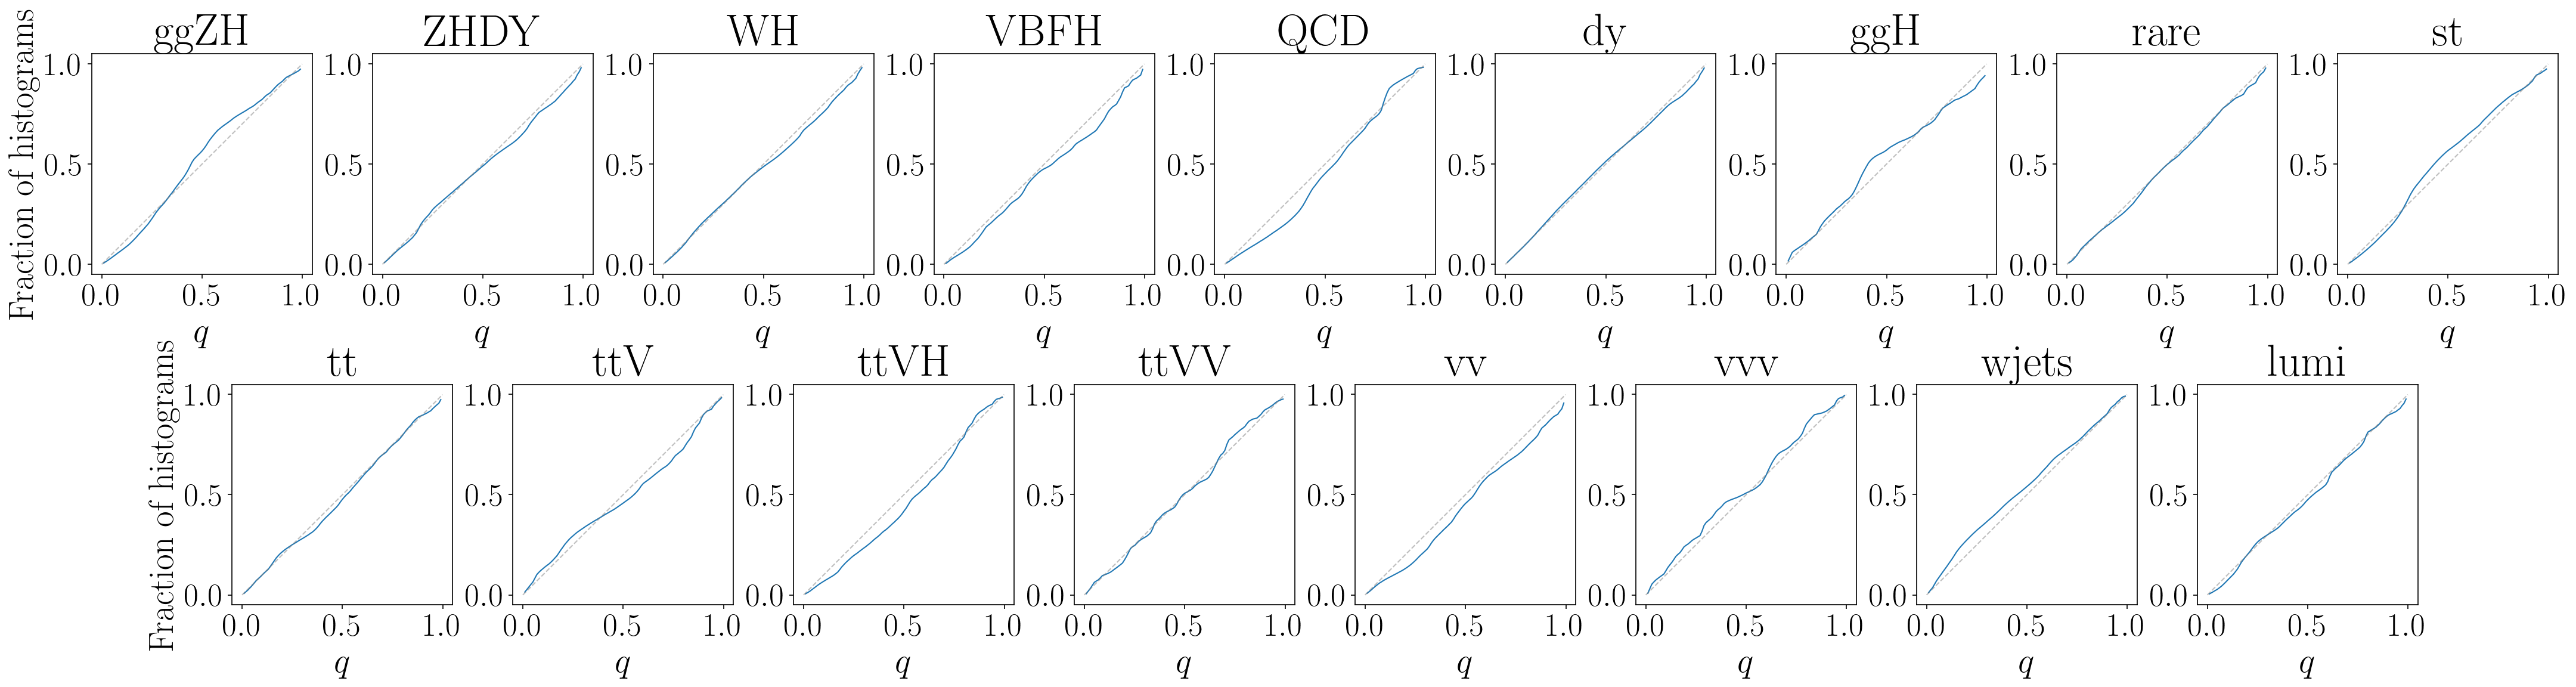
\includegraphics[width=\linewidth]{figures/inference/ecal}
	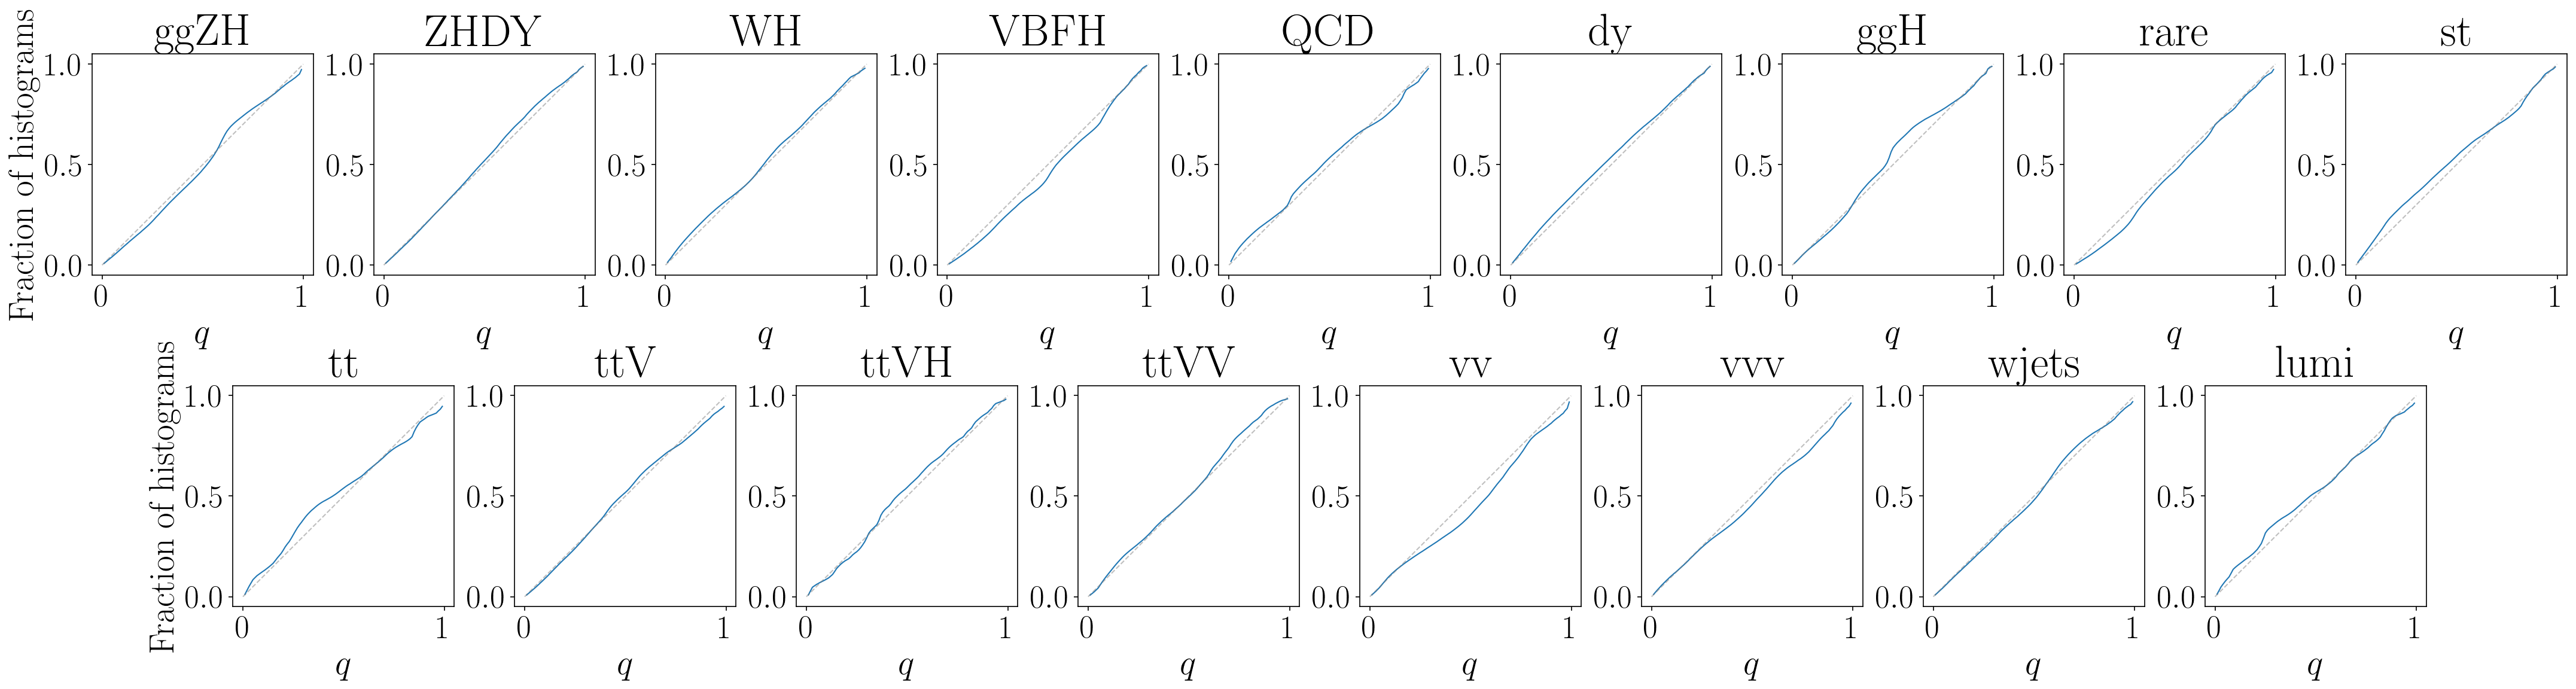
\includegraphics[width=\linewidth]{figures/inference/ecal_SN}
	\caption{\textcolor{red}{Need to be updated!} The calibration curves for the "pure" cINN and summary network-extended cINN. Note the closeness to the perfect calibration curve shown in the gray dashed line.}
	\label{fig:ecals}
\end{figure}

A natural measure to describe how strongly these biases are present in the network is the meadian calibration error, defined as

\begin{equation*}
	e^{med}_{cal} = \underset{q}{\text{med}} \left|\frac{N^q_{in}}{N} - q\right|
\end{equation*}

describing the median absolute distance of the histogram ratios to the ideal case (where this ratio equals $q$). These values for both networks have been listed in tab. \ref{tab:ecal_med}. As it can be seen from the table all of these values are $e^{med}_{cal}\lesssim\mathcal{O}(0.04)$. With such small mean deviations and calibration curves being close to the perfect calibration line, the resulting network model has no significant inherent biases (due to wrong initialization or other nontrivial effects).

\begin{table}[h!]
	\centering
	\begin{tabular}{ccc}
		\multirow{2}{*}{Process}& \multicolumn{2}{c}{$e^{med}_{cal}$} \\
		 & cINN & SN-cINN \\
		\hline
		\texttt{ggZH }   & 0.0156    &    0.0258  \\
		\texttt{ZHDY }   & 0.0299    &    0.0103  \\
		\texttt{WH   }   & 0.0148    &    0.0176  \\
		\texttt{VBFH }   & 0.0256    &    0.0428  \\
		\texttt{QCD  }   & 0.0147    &    0.0285  \\
		\texttt{dy   }   & 0.0133    &    0.0323  \\
		\texttt{ggH  }   & 0.0395    &    0.0183  \\
		\texttt{rare }   & 0.0399    &    0.0261  \\
		\texttt{st   }   & 0.0229    &    0.0323  \\
		\texttt{tt   }   & 0.0101    &    0.0300  \\
		\texttt{ttV  }   & 0.0212    &    0.0144  \\
		\texttt{ttVH }   & 0.0159    &    0.0227  \\
		\texttt{ttVV }   & 0.0403    &    0.0146  \\
		\texttt{vv   }   & 0.0333    &    0.0441  \\
		\texttt{vvv  }   & 0.0326    &    0.0331  \\
		\texttt{wjets}   & 0.0070    &    0.0127  \\
		\texttt{lumi }   & 0.0156    &    0.0248  \\
		\hline
	\end{tabular}
	\caption{The median calibration errors for the cINN and the summary network-extended (SN-cINN).}
	\label{tab:ecal_med}
\end{table}

\Subsection{\textcolor{red}{Network Predictions}}

The predictions for the complete test dataset are shown in fig. \ref{fig:predictions}. For each two dimensional histogram, the x axis shows the predicted values for a parameter on the y axis. In these plots several structures are clearly visible, which can be categorised into three groups for both networks:

\begin{itemize}
	\item[] \textit{Unrecognised processes} are those, where the network has clear difficulties obtaining the parameter with which the processes had been scaled. These are \texttt{VBFH, ggH, ttVH, ttVV, vvv} all of which are rare background processes. Due to the network not being able to differentiate between the different scalings, all of these are fitted close to the mean of the prior distribution, resulting in the thin vertical distribution in fig. \ref{fig:predictions}. \textcolor{red}{looking at the DNN score histograms}
	\item[] \textit{Weakly recognised processes} are \texttt{rare}, \texttt{ttV}, \texttt{vv}. For these processes, the network can already resolve sevaral parameters close to the mean, from where the sensitivity starts to develop during training. Parameters further away from the mean are still fit the average value, resulting in an overall lense-like shape.
	\item[] \textit{Recongnised processes} are all signal processes \texttt{ggZH}, \texttt{ZHDY} and \texttt{WH} and the major background sources \texttt{QCD}, \texttt{dy}, \texttt{st}, \texttt{tt}, \texttt{wjets}. For these processes, most scaling parameters predictions lie close to the real value, hence distribution scatter around the "perfect prediction diagonal".
\end{itemize}

Note the unique decrease in sensitivity for the signal processes \texttt{ggZH}, \texttt{ZHDY} and \texttt{WH} for $\mu\lesssim10$ resulting in a tail-like structure stretching towards the mean. Uniquely to these processes, the network cannot resolve them as long as the signal strength modifier parameters lie below a certain threshold value for some configurations. Since their contribution (compared to the other significant background processes) is already low, the added statistical and systematic effects (the Poisson bin-variation being the most significant one, as it modifies all bins with $\sqrt{N}$) renders these statistically undetectable.

Note that the calibration curves show no signs of inherent biases in the resulting model, hence the fact that this effect is due to some training relics can be excluded. It is expected then, that the posterior distributions are broader in this range covering the true value, which will be discussed in the next section.

In general, this resolution effect only be can further tackled by a more refined event selection and/or category creation and similar improved analysis techniques.

\begin{figure}[h!]
	\centering
	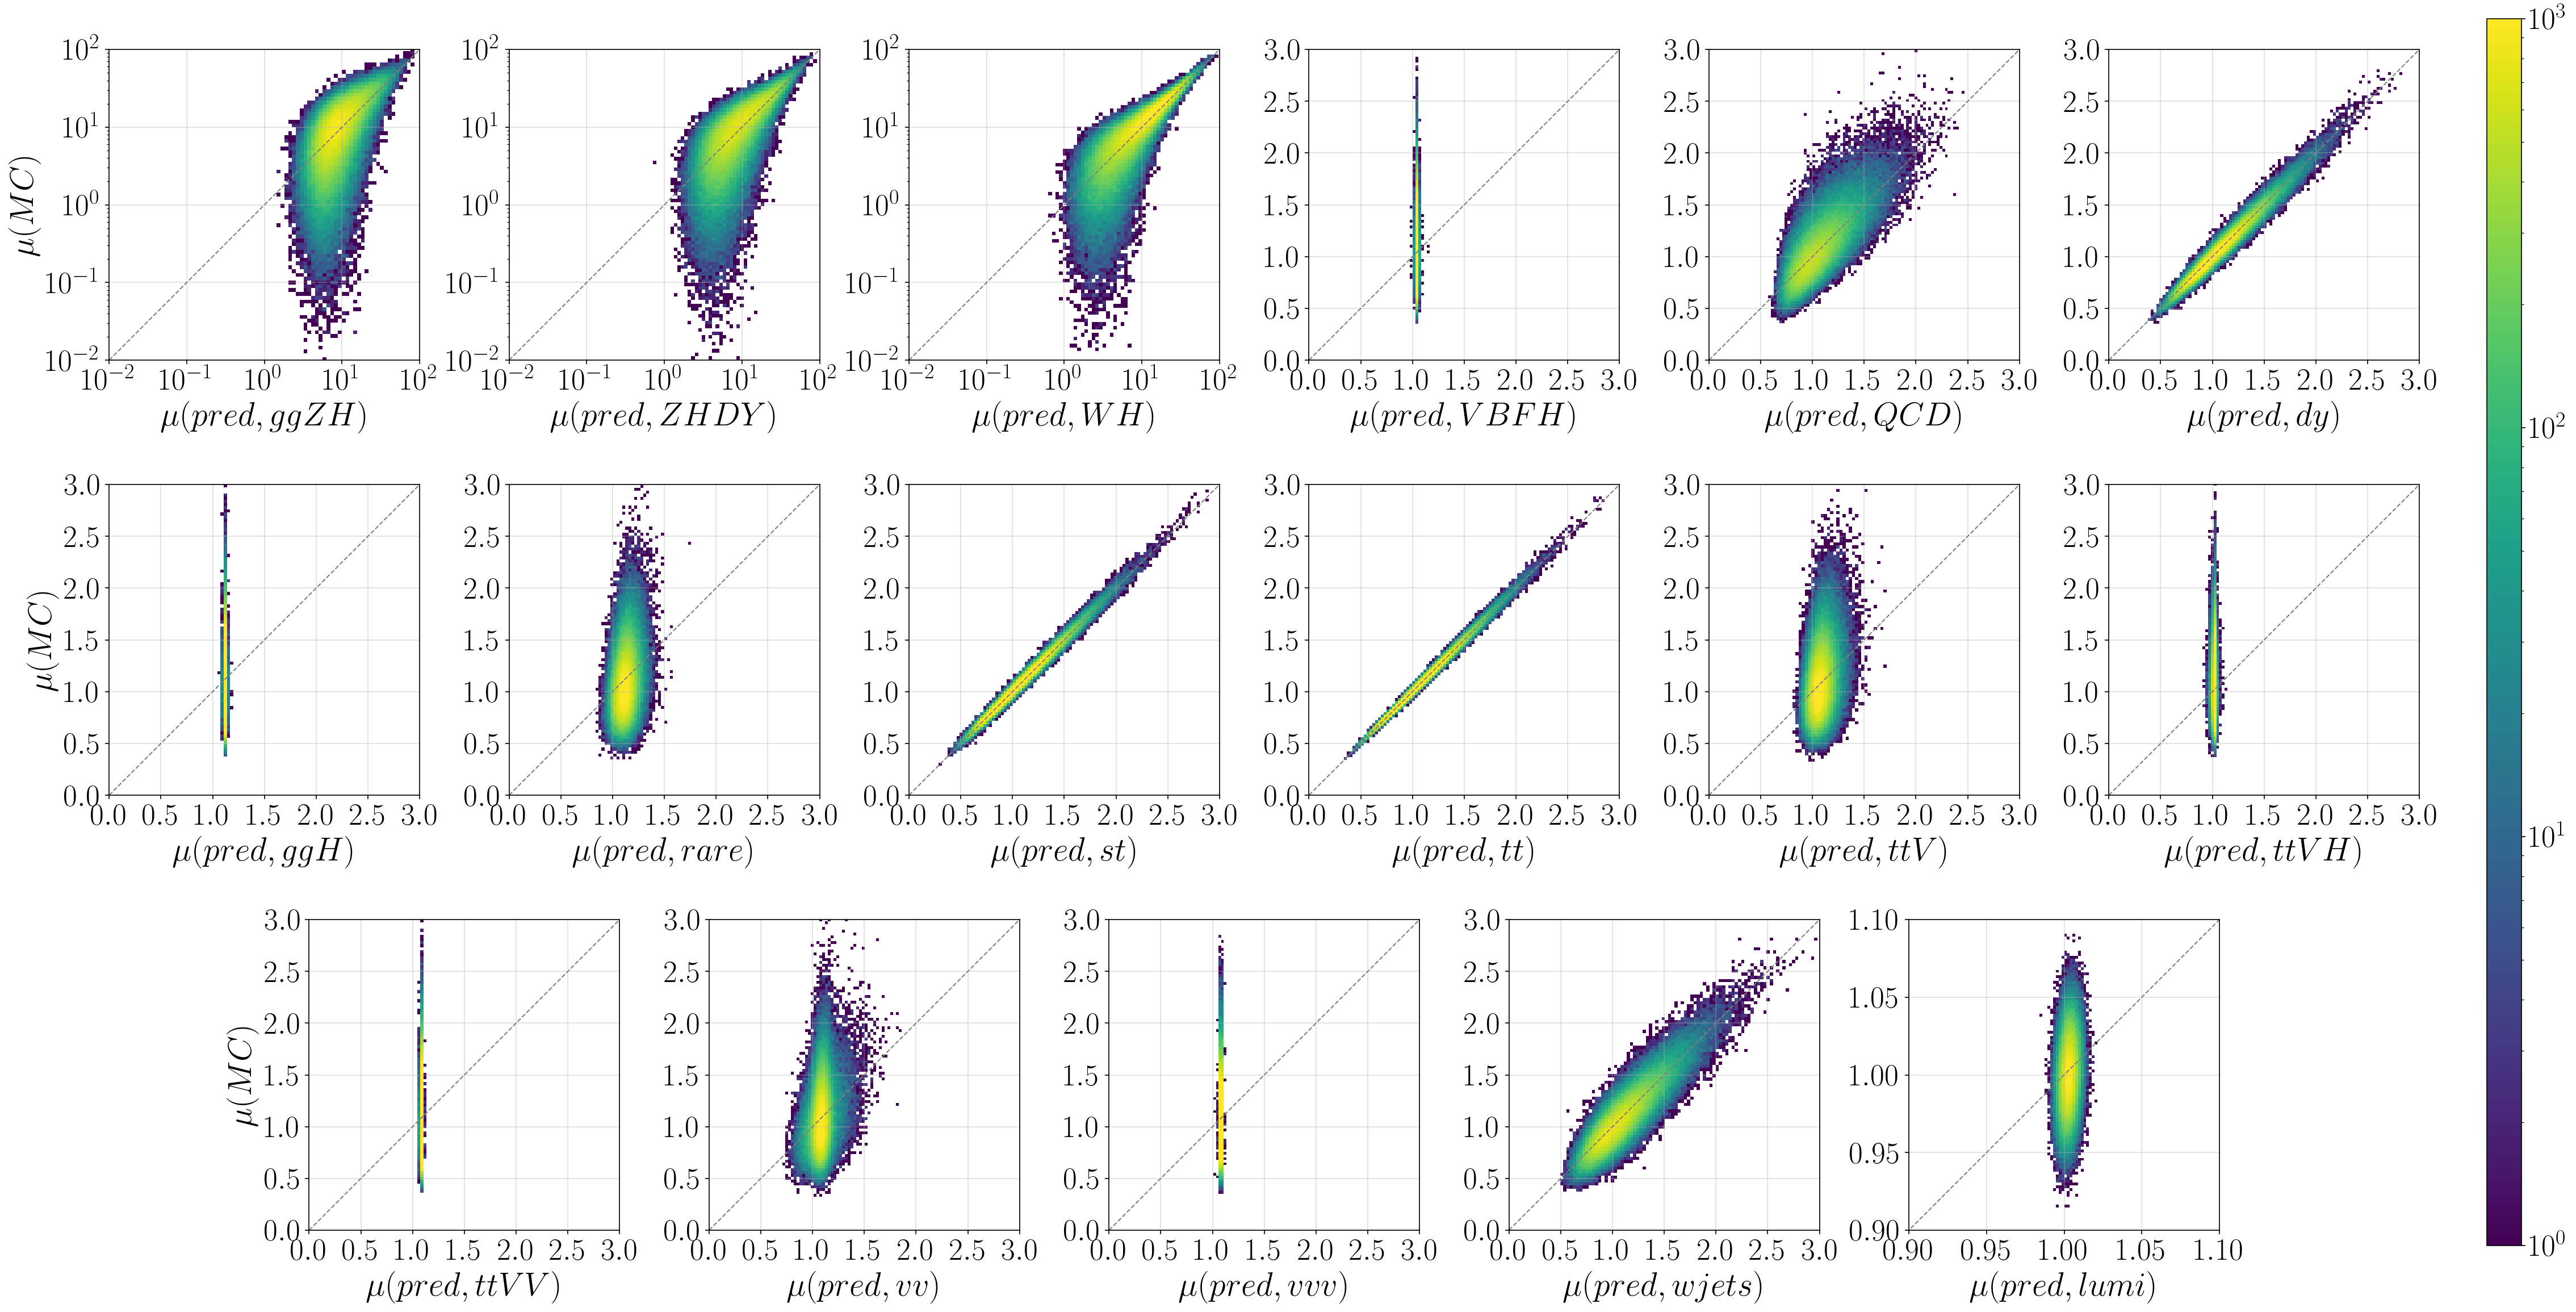
\includegraphics[width=\linewidth]{figures/inference/p}
	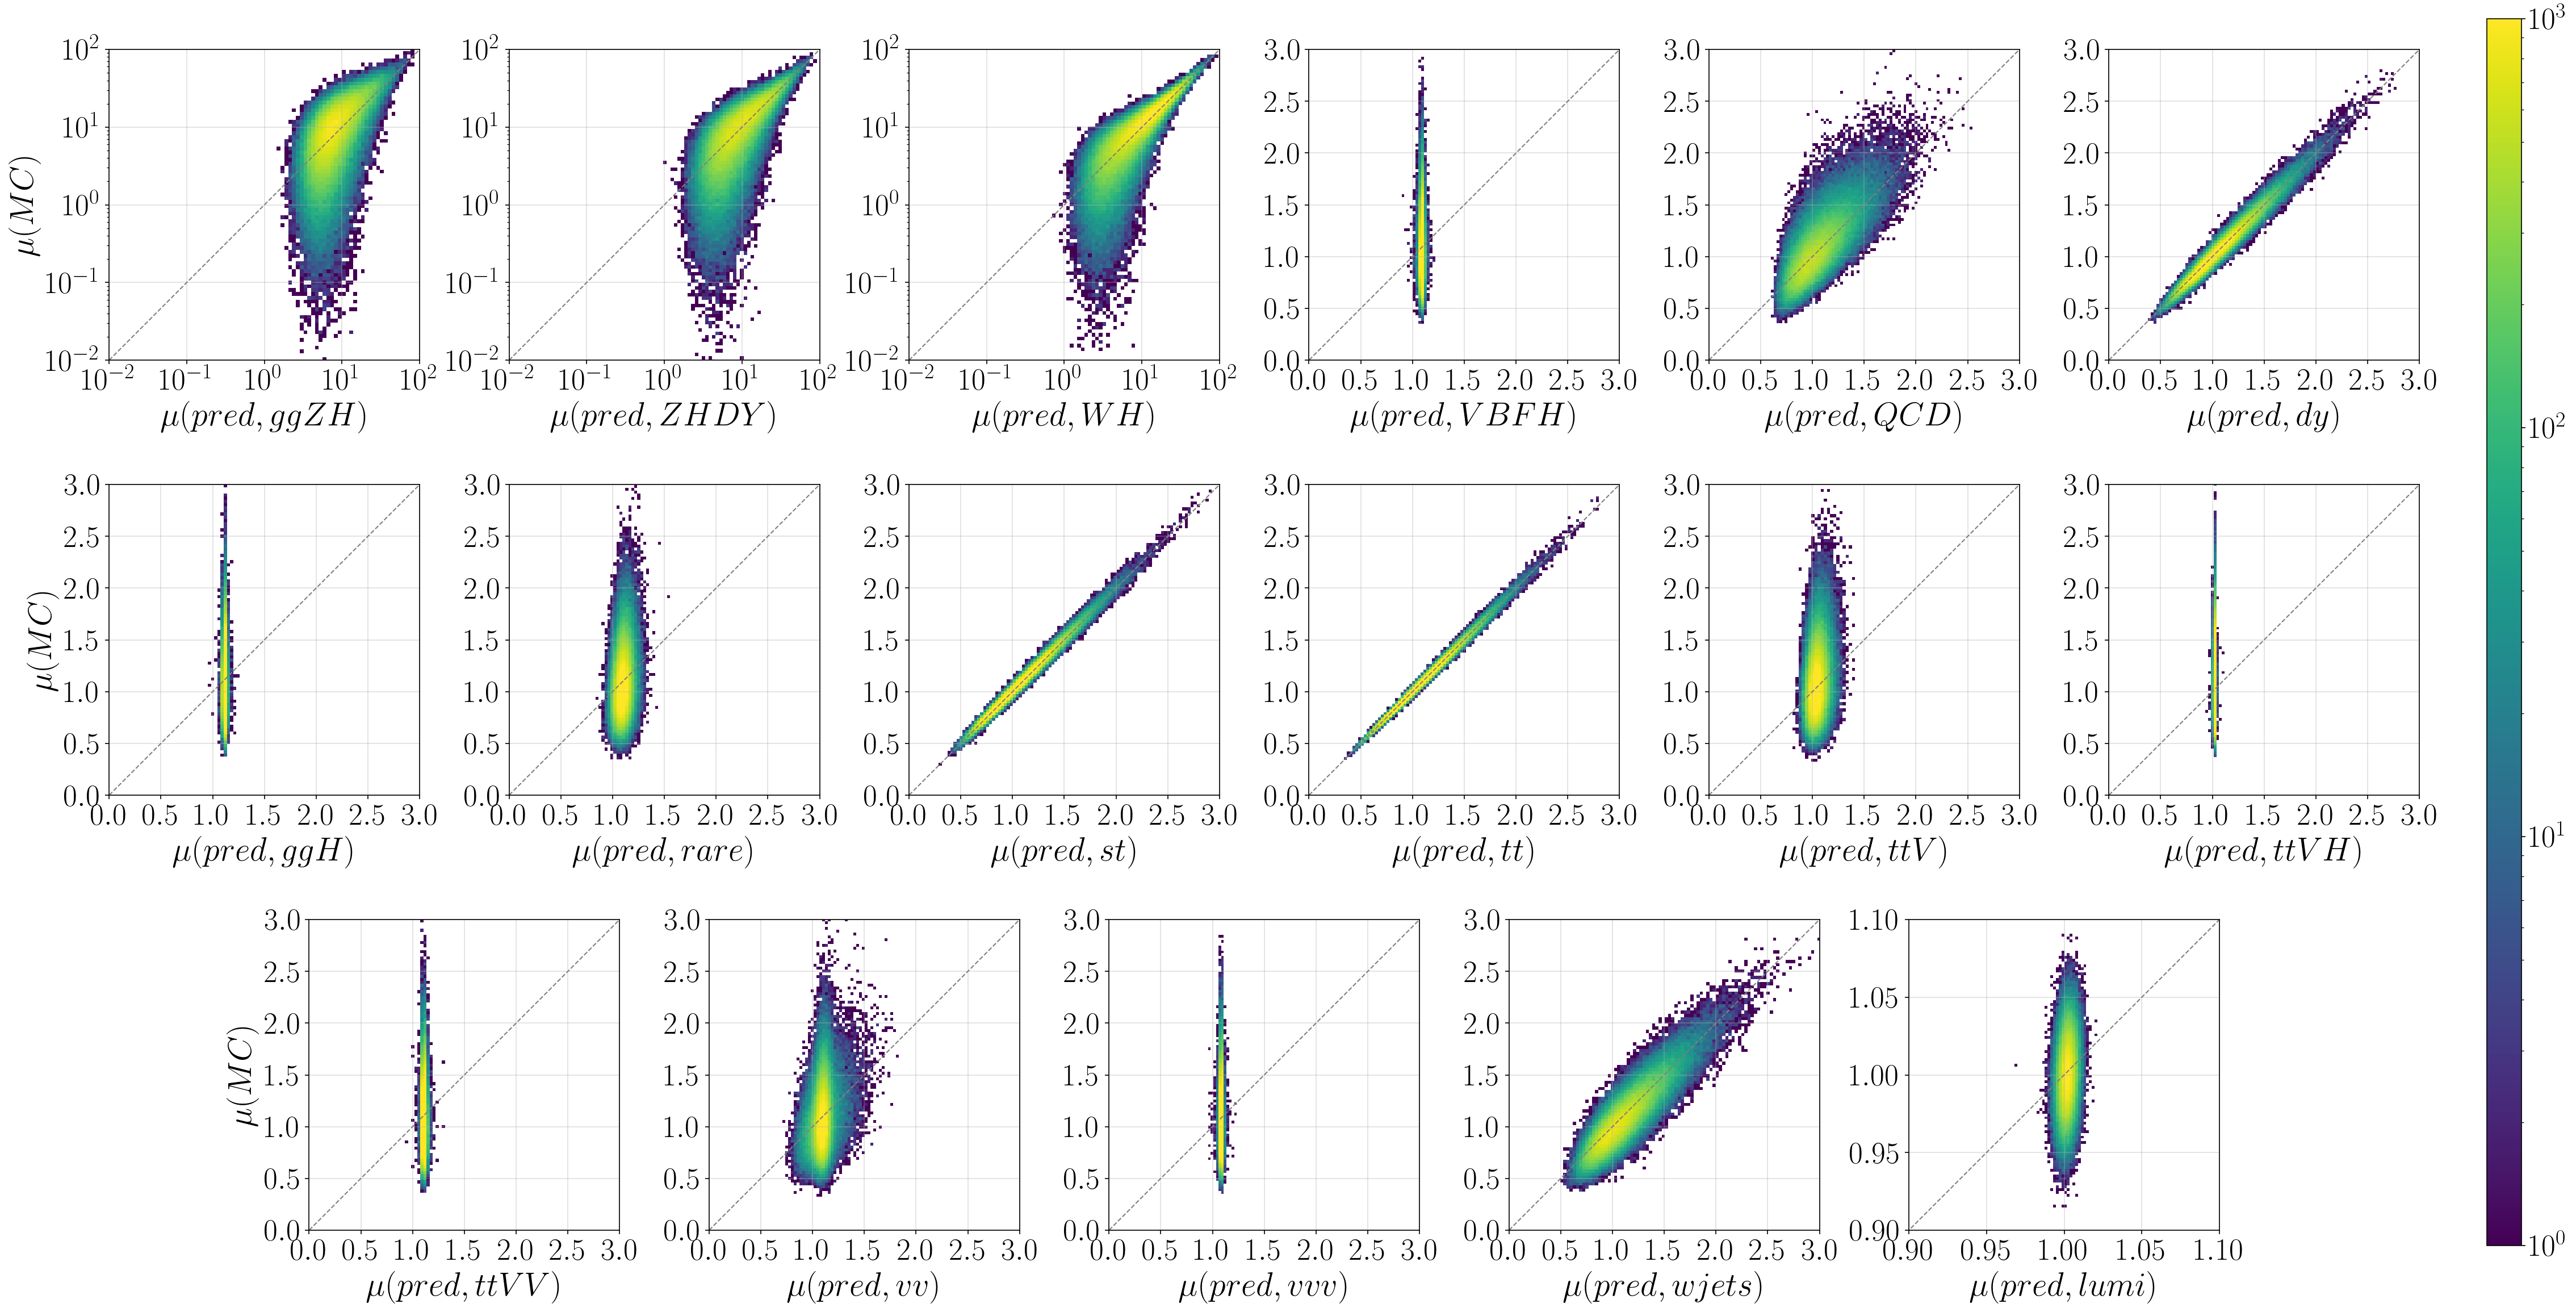
\includegraphics[width=\linewidth]{figures/inference/p_SN}
	\caption{The predicted signal scale parameters vs. the simulated "real" Monte Carlo values. Note the three main }
	\label{fig:predictions}
\end{figure}

\Subsection{Posterior Inference}

Following the sampling from the target Gaussian function in the latent space, the posteriors can be inferred for the physics parameters for both networks. These are shown in fig. \ref{fig:posteriors} for the nominal histogram where all expectations are $\mu=1$. \footnote{Can be understood as inference on an Asimov datasets.} The obtained posterior distributions (normalized to 1) are shown in blue with their means (the predictions) drawn in black. The true values are shown with the red line. The edges of the 68\% quantiles are drawn in black; these can be interpreted as the uncertainty on the scaling parameters. The original posterior distributions for the signal modifier parameters and the nuisance parameters are shown in orange.

\begin{figure}[h!]
	\centering
	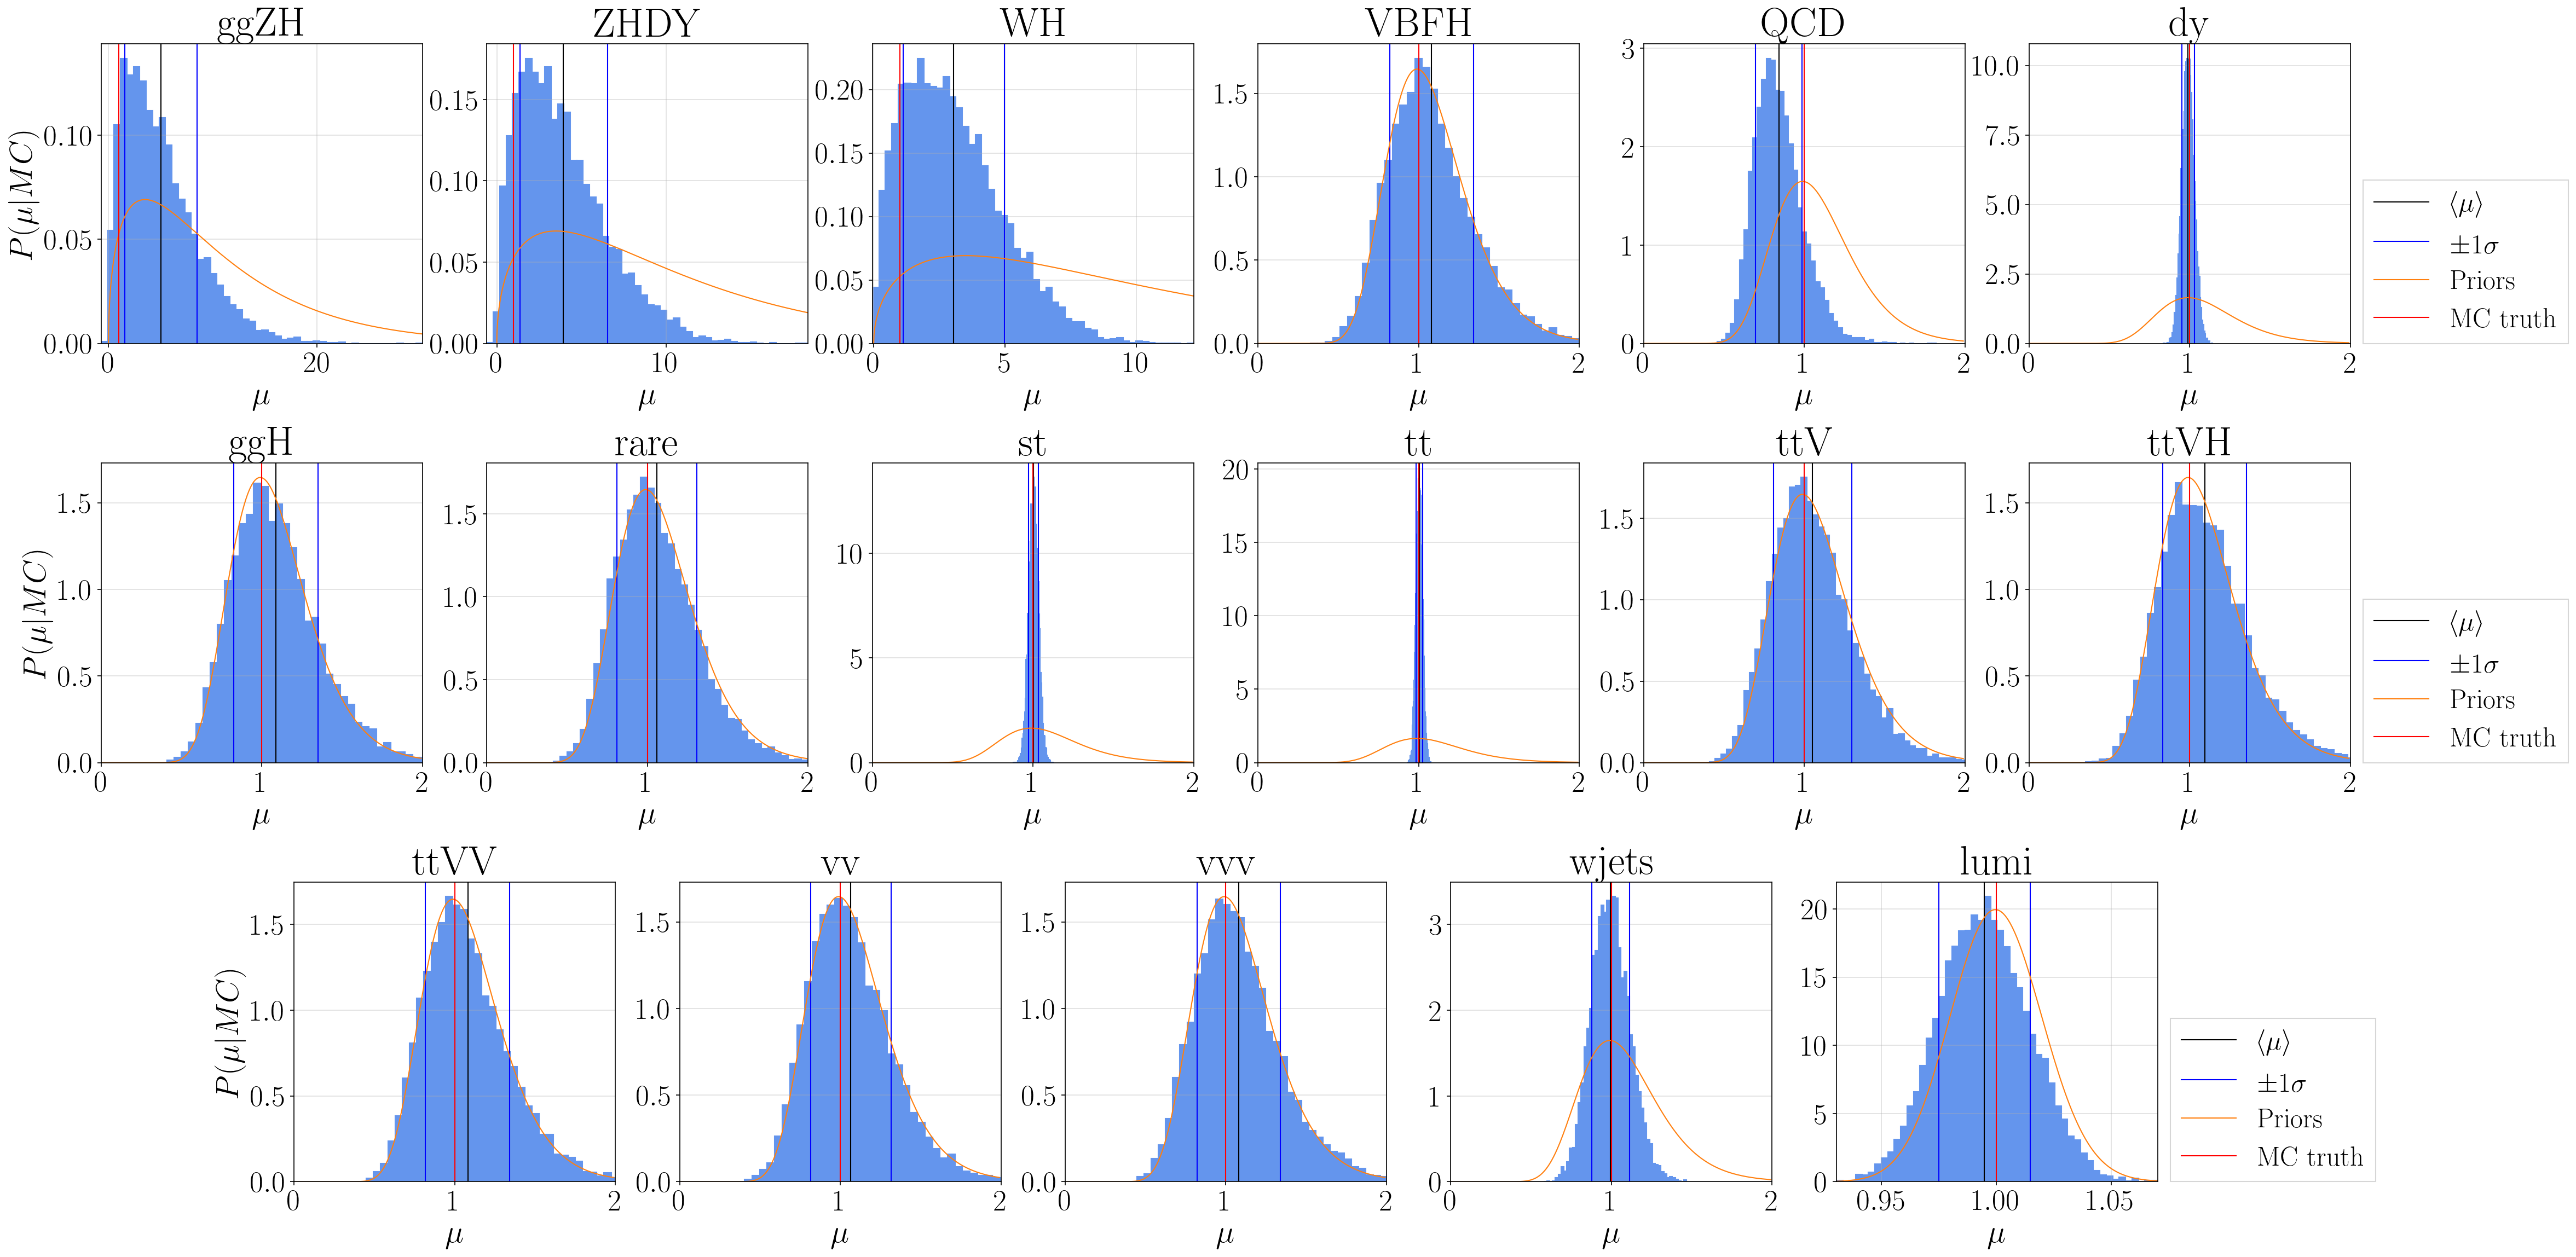
\includegraphics[width=\linewidth]{figures/inference/finalNoSummarye11000_posteriors}
	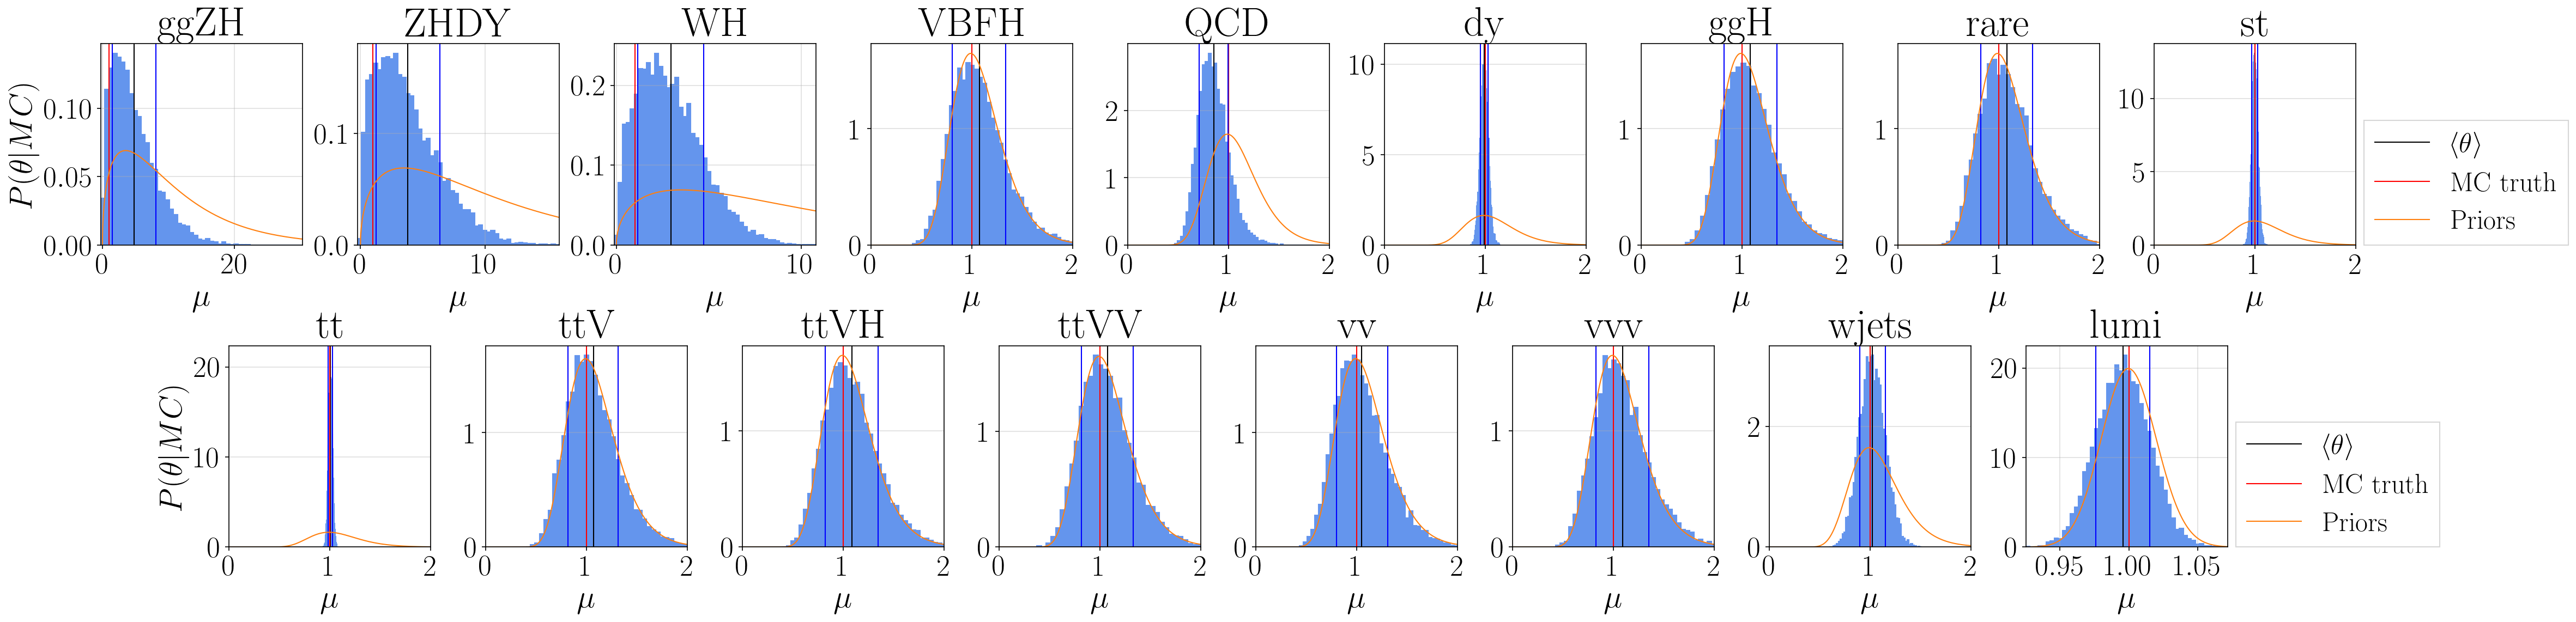
\includegraphics[width=\linewidth]{figures/inference/finalSummary1Layer11000e300NodesCdim100_posteriors}
	\caption{The posterior distributions for each process.}
	\label{fig:posteriors}
\end{figure}

Both networks succeed in the reconstruction of the nominal parameters with differing precision. It appears at first glance that the some recongnized background processes (\texttt{dy}, \texttt{st}, \texttt{tt}) have an order of magnitude narrower posterior distribution. From the posterior estimation, such behaviour is expected as the calibration curves show no signs of biases, meaning the posteriors should all be scattered around the true values with their widths covering it. This implies the network sensitivity can only be characterized by the width of the posterior distributions for well-behaving (single-peaked) posteriors; in other words, enhanced sensitivity implies narrower posteriors.

All three signal processes are overestimated with the true values lying closely outside of the 68\% quantiles. All background scaling parameters (except for \texttt{QCD}, which is underestimated and lies outside of the $1\sigma$ range) lie close to their nominal values.

For weakly recognized and unrecognized processes, an interesting property of cINNs can be observed. Taking a glimpse at the blue posteriors and the orange analytic prior distributions for any of these processes (\texttt{VBHF, ggH, rare, ttV, ttVH, ttVV, vv, vvv}) only minimal changes in the former can be observed. For the cINN, these processes are statistically independent of the posteriors (and therefore, redundant in a way), so the normalizing flow mapping the priors to the Gaussian distributions does not need to decorrelate them from the other observables (which, in reality, should be done, but their contribution appears negligible at the current sensitivity), as they -- from the network's perspective -- have no influence on the conditions whatsoever.

Mathematically speaking, if some physics observations $y$ are independent of a phyics parameter $x$, it means that by Bayes' Theorem the posteriors can be rewritten using the priors $p(x)$ as

\begin{equation*}
	p(x|y) = \frac{p(y|x)p(x)}{p(y)} = \frac{\cancel{p(y)}}{\cancel{p(y)}} p(x)
\end{equation*}

Which means the posteriors and the priors coincide. Note that the independence should be mutual, so the probability of obtaining $x$ given $y$ does not change either, directly yielding $p(x|y) = p(x)$. Hence, the blue histograms coincide with the orange priors.

This observation shows the "naked" presence of the normalizing flow itself. The NF maps the datapoints from the prior distributions to a normal distribution via a diffeomorphism while the network is trained to optimize the modelled posterior distributions with respect to the unknown real distribution. From the results above, it becomes less surprising to observe that the network is capable of reproducing the priors for parameters which are independent of the conditions --- from a single condition and samples from the latent space distribution alone.

The numerical results for the inference have been summarized in tab. \ref{tab:inference_res}.

\begin{table}[h!]
	\centering
	\begin{tabular}{cccc}
		\multirow{2}{*}{Processes} & \multicolumn{3}{c}{$\mu$} \\
		 & cINN & SN-cINN & \texttt{CMSCombine} \\
		 \hline\\
		$\mu_\text{ggZH } $ & $5.10^{+3.57}_{-3.50}$ & $4.86^{+3.38}_{-3.33}$ &  \textcolor{red}{combine}  \\[0.3em]
		$\mu_\text{ZHDY } $ & $3.90^{+2.62}_{-2.57}$ & $3.76^{+2.57}_{-2.52}$ &    \\[0.3em]
		$\mu_\text{WH   } $ & $3.02^{+1.92}_{-1.90}$ & $2.93^{+1.80}_{-1.80}$ &    \\[0.3em]
		$\mu_\text{VBFH } $ & $1.08^{+0.27}_{-0.27}$ & $1.08^{+0.26}_{-0.26}$ & -- \\[0.3em]
		$\mu_\text{QCD  } $ & $0.84^{+0.14}_{-0.14}$ & $0.86^{+0.15}_{-0.15}$ & -- \\[0.3em]
		$\mu_\text{dy   } $ & $0.99^{+0.04}_{-0.04}$ & $0.99^{+0.04}_{-0.04}$ & -- \\[0.3em]
		$\mu_\text{ggH  } $ & $1.09^{+0.27}_{-0.27}$ & $1.08^{+0.26}_{-0.26}$ & -- \\[0.3em]
		$\mu_\text{rare } $ & $1.06^{+0.25}_{-0.25}$ & $1.08^{+0.26}_{-0.26}$ & -- \\[0.3em]
		$\mu_\text{st   } $ & $1.00^{+0.03}_{-0.03}$ & $1.00^{+0.03}_{-0.03}$ & -- \\[0.3em]
		$\mu_\text{tt   } $ & $1.00^{+0.02}_{-0.02}$ & $1.00^{+0.02}_{-0.02}$ & -- \\[0.3em]
		$\mu_\text{ttV  } $ & $1.05^{+0.24}_{-0.24}$ & $1.07^{+0.25}_{-0.25}$ & -- \\[0.3em]
		$\mu_\text{ttVH } $ & $1.09^{+0.27}_{-0.27}$ & $1.08^{+0.27}_{-0.27}$ & -- \\[0.3em]
		$\mu_\text{ttVV } $ & $1.08^{+0.26}_{-0.27}$ & $1.07^{+0.26}_{-0.26}$ & -- \\[0.3em]
		$\mu_\text{vv   } $ & $1.06^{+0.25}_{-0.25}$ & $1.06^{+0.25}_{-0.25}$ & -- \\[0.3em]
		$\mu_\text{vvv  } $ & $1.09^{+0.27}_{-0.27}$ & $1.09^{+0.27}_{-0.27}$ & -- \\[0.3em]
		$\mu_\text{wjets} $ & $0.99^{+0.12}_{-0.12}$ & $1.02^{+0.13}_{-0.13}$ & -- \\[0.3em]
		$\mu_\text{lumi } $ & $1.00^{+0.02}_{-0.02}$ & $1.00^{+0.02}_{-0.02}$ & -- \\[0.3em]
		\hline
	\end{tabular}
	\caption{The predicted values of the signal strength modifier and of the nuisance parameter for the cINN and the summary-network extended network (SN-cINN). Note the similarity of the output of both networks.}
	\label{tab:inference_res}
\end{table}